\documentclass[tikz,border=3pt]{standalone}
\usetikzlibrary{arrows.meta,positioning,shapes.multipart,shapes.symbols,shapes.geometric,calc}
\tikzset{
  entity/.style     = {rectangle,draw,rounded corners,align=center,font=\small,minimum width=2.8cm,minimum height=1.0cm},
  datastore/.style  = {cylinder,aspect=0.3,draw,align=center,font=\small,minimum width=2.8cm,minimum height=1.0cm},
  process/.style    = {ellipse,draw,align=center,font=\small,minimum width=3cm,minimum height=1cm},
  flow/.style       = {-Latex,thick},
}
\begin{document}
%% Level 0 DFD
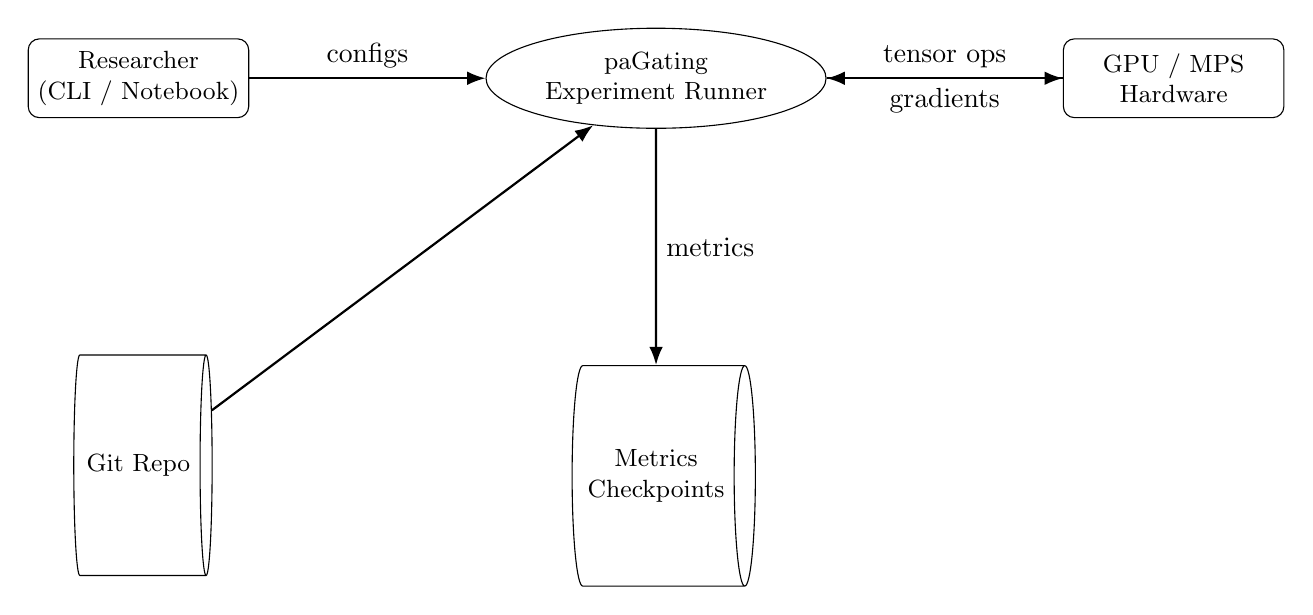
\begin{tikzpicture}[node distance=3cm]
\node[entity]  (user)    {Researcher\\(CLI / Notebook)};
\node[process] (runner)  [right=of user] {paGating\\Experiment Runner};
\node[datastore] (logs)  [below=of runner] {Metrics \\ Checkpoints};
\node[entity]  (gpu)   [right=of runner] {GPU / MPS\\Hardware};
\node[datastore] (repo) [below=of user] {Git Repo};
\draw[flow] (user) -- node[above]{configs} (runner);
\draw[flow] (runner) -- node[above]{tensor ops} (gpu);
\draw[flow] (gpu) -- node[below]{gradients} (runner);
\draw[flow] (runner) -- node[right]{metrics} (logs);
\draw[flow] (repo) -- (runner);
\end{tikzpicture}
\end{document} 